\documentclass[a0paper,portrait]{baposter}

\usepackage{lipsum}          % This is just for some blindtext
\usepackage{biblatex}
\usepackage{relsize}	       % For \smaller
\usepackage{url}			       % For \url
\usepackage{epstopdf}	       % Included EPS files automatically converted to PDF to include with pdflatex
\usepackage{multicol}        % Multi Columns

\usepackage{amsmath} % math
\usepackage{amssymb}
\usepackage{accents}
\usepackage[slovak]{babel}
\usepackage{csquotes}
\usepackage{xcolor}
\usepackage{marvosym}


%%%%%%%%%%%%%%%%%%%%%%%%%%%%%%%%%%%%%%%%%%%%%%%%%%%%%%%%%%%%%%%%%%%%%%%%%%%%%%%%
%%% Utility functions %%%%%%%%%%%%%%%%%%%%%%%%%%%%%%%%%%%%%%%%%%%%%%%%%%%%%%%%%%
%%%%%%%%%%%%%%%%%%%%%%%%%%%%%%%%%%%%%%%%%%%%%%%%%%%%%%%%%%%%%%%%%%%%%%%%%%%%%%%%

%%% Save space in lists. Use this after the opening of the list %%%%%%%%%%%%%%%%
\renewcommand{\vec}[1]{\bm{#1}}
%\renewcommand{\dot}[1]{\accentset{\cdot}{#1}}
\renewcommand{\ddot}[1]{\stackrel{..}{#1}}
%\newcommand{\tildeI}[1]{\overset{\tilde{}}{#1}} 

%\renewcommand{\bibname}{}

\newcommand{\vnabla}{\vec{\nabla}}

\renewcommand{\d}[1]{\text{d} #1}
\newcommand{\dxx}{\,\text{d}\vec{x}}
\newcommand{\dx}{\,\text{d}x}

\newcommand{\diff}[2]{\frac{\text{d}#1}{\text{d}#2}}
\newcommand{\idiff}[2]{\text{d}#1 / \text{d}#2}
\newcommand{\pdiff}[2]{\frac{\partial #1}{\partial #2}}
\newcommand{\pdifff}[2]{\frac{\partial^2 #1}{\partial #2^2}}
\newcommand{\ipdiff}[2]{\partial #1 / \partial #2}
\newcommand{\vdiff}[2]{\frac{\delta #1}{\delta #2}}
\newcommand{\ivdiff}[2]{\delta #1 / \delta #2}

\definecolor{mcr_purple}{RGB}{108,44,145}

%%%%%%%%%%%%%%%%%%%%%%%%%%%%%%%%%%%%%%%%%%%%%%%%%%%%%%%%%%%%%%%%%%%%%%%%%%%%%%%
%%% Document Start %%%%%%%%%%%%%%%%%%%%%%%%%%%%%%%%%%%%%%%%%%%%%%%%%%%%%%%%%%%%
%%%%%%%%%%%%%%%%%%%%%%%%%%%%%%%%%%%%%%%%%%%%%%%%%%%%%%%%%%%%%%%%%%%%%%%%%%%%%%%

\begin{document}
\typeout{Poster rendering started}

%%% General Poster Settings %%%%%%%%%%%%%%%%%%%%%%%%%%%%%%%%%%%%%%%%%%%%%%%%%%%
%%%%%% Eye Catcher, Title, Authors and University Images %%%%%%%%%%%%%%%%%%%%%%
\begin{poster}{
  columns=2,
	grid=false,
	borderColor=uniblue,
	headerColorOne=uniblue,
	headerColorTwo=uniblue,
	headerFontColor=white,
  headerheight=14em,
	boxColorOne=white,
  boxpadding=1em,
	headershape=rounded,
	headerfont=\Large\textsf,
	textborder=rounded,
	background=shadetb,
  bgColorOne=uniblue!10,
  bgColorTwo=uniblue!30,
	headerborder=open,
  boxshade=plain,
  eyecatcher=false
}
%%% Eye Cacther %%%%%%%%%%%%%%%%%%%%%%%%%%%%%%%%%%%%%%%%%%%%%%%%%%%%%%%%%%%%%%%
{ %\vspace{1em}
}
%%% Title %%%%%%%%%%%%%%%%%%%%%%%%%%%%%%%%%%%%%%%%%%%%%%%%%%%%%%%%%%%%%%%%%%%%%
{\vspace{1.25em} 
\smaller This is the unnecessarily complicated poster title}
%%% Authors %%%%%%%%%%%%%%%%%%%%%%%%%%%%%%%%%%%%%%%%%%%%%%%%%%%%%%%%%%%%%%%%%%%
{
  \vspace{1em}
  {Jakub \v{S}\v{t}avina\textsuperscript{\Letter}}, Other Student \\
	{\smaller \smaller Department of Physics and Astronomy, The University of Manchester, Manchester, United Kingdom \vspace{1em}} \\ \textcolor{black}{\smaller {\Letter~e-mail: jakub.stavina@student.manchester.ac.uk} \\
\textcolor{mcr_purple}{\smaller Here we add some further info., module name, module number, hyperlinks, etc.}
}}
%%% Logo %%%%%%%%%%%%%%%%%%%%%%%%%%%%%%%%%%%%%%%%%%%%%%%%%%%%%%%%%%%%%%%%%%%%%%
{\begin{minipage}{18.0em}
    
\includegraphics[height=7.5em]{logo-uni.pdf}
  \end{minipage}}

%%% Abstract %%%%%%%%%%%%%%%%%%%%%%%%%%%%%%%%%%%%%%%%%%%%%%%%%%%%%%%%%%%%%%%%%%
\headerbox{Abstract}{name=abstract,column=0,row=0,span=2}{
%\begin{multicols}{2} 
    Lorem ipsum dolor sit amet, consectetur adipiscing elit, sed do eiusmod tempor incididunt ut labore et dolore magna aliqua. Ut enim ad minim veniam, quis nostrud exercitation ullamco laboris nisi ut aliquip ex ea commodo consequat. Duis aute irure dolor in reprehenderit in voluptate velit esse cillum dolore eu fugiat nulla pariatur. Excepteur sint occaecat cupidatat non proident, sunt in culpa qui officia deserunt mollit anim id est laborum.

%\end{multicols}
}

%%% Box 1 %%%%%%%%%%%%%%%%%%%%%%%%%%%%%%%%%%%%%%%%%%%%%%%%%%%%%%%%%%%%%%%%%%%%%
\headerbox{What is going on?}{name=box1,column=0,below=abstract%,above=bottom
}{Lorem ipsum dolor sit amet, consectetur adipiscing elit, sed do eiusmod tempor incididunt ut labore et dolore magna aliqua. Ut enim ad minim veniam, quis nostrud exercitation ullamco laboris nisi ut aliquip ex ea commodo consequat. Duis aute irure dolor in reprehenderit in voluptate velit esse cillum dolore eu fugiat nulla pariatur. Excepteur sint occaecat cupidatat non proident, sunt in culpa qui officia deserunt mollit anim id est laborum.
 
  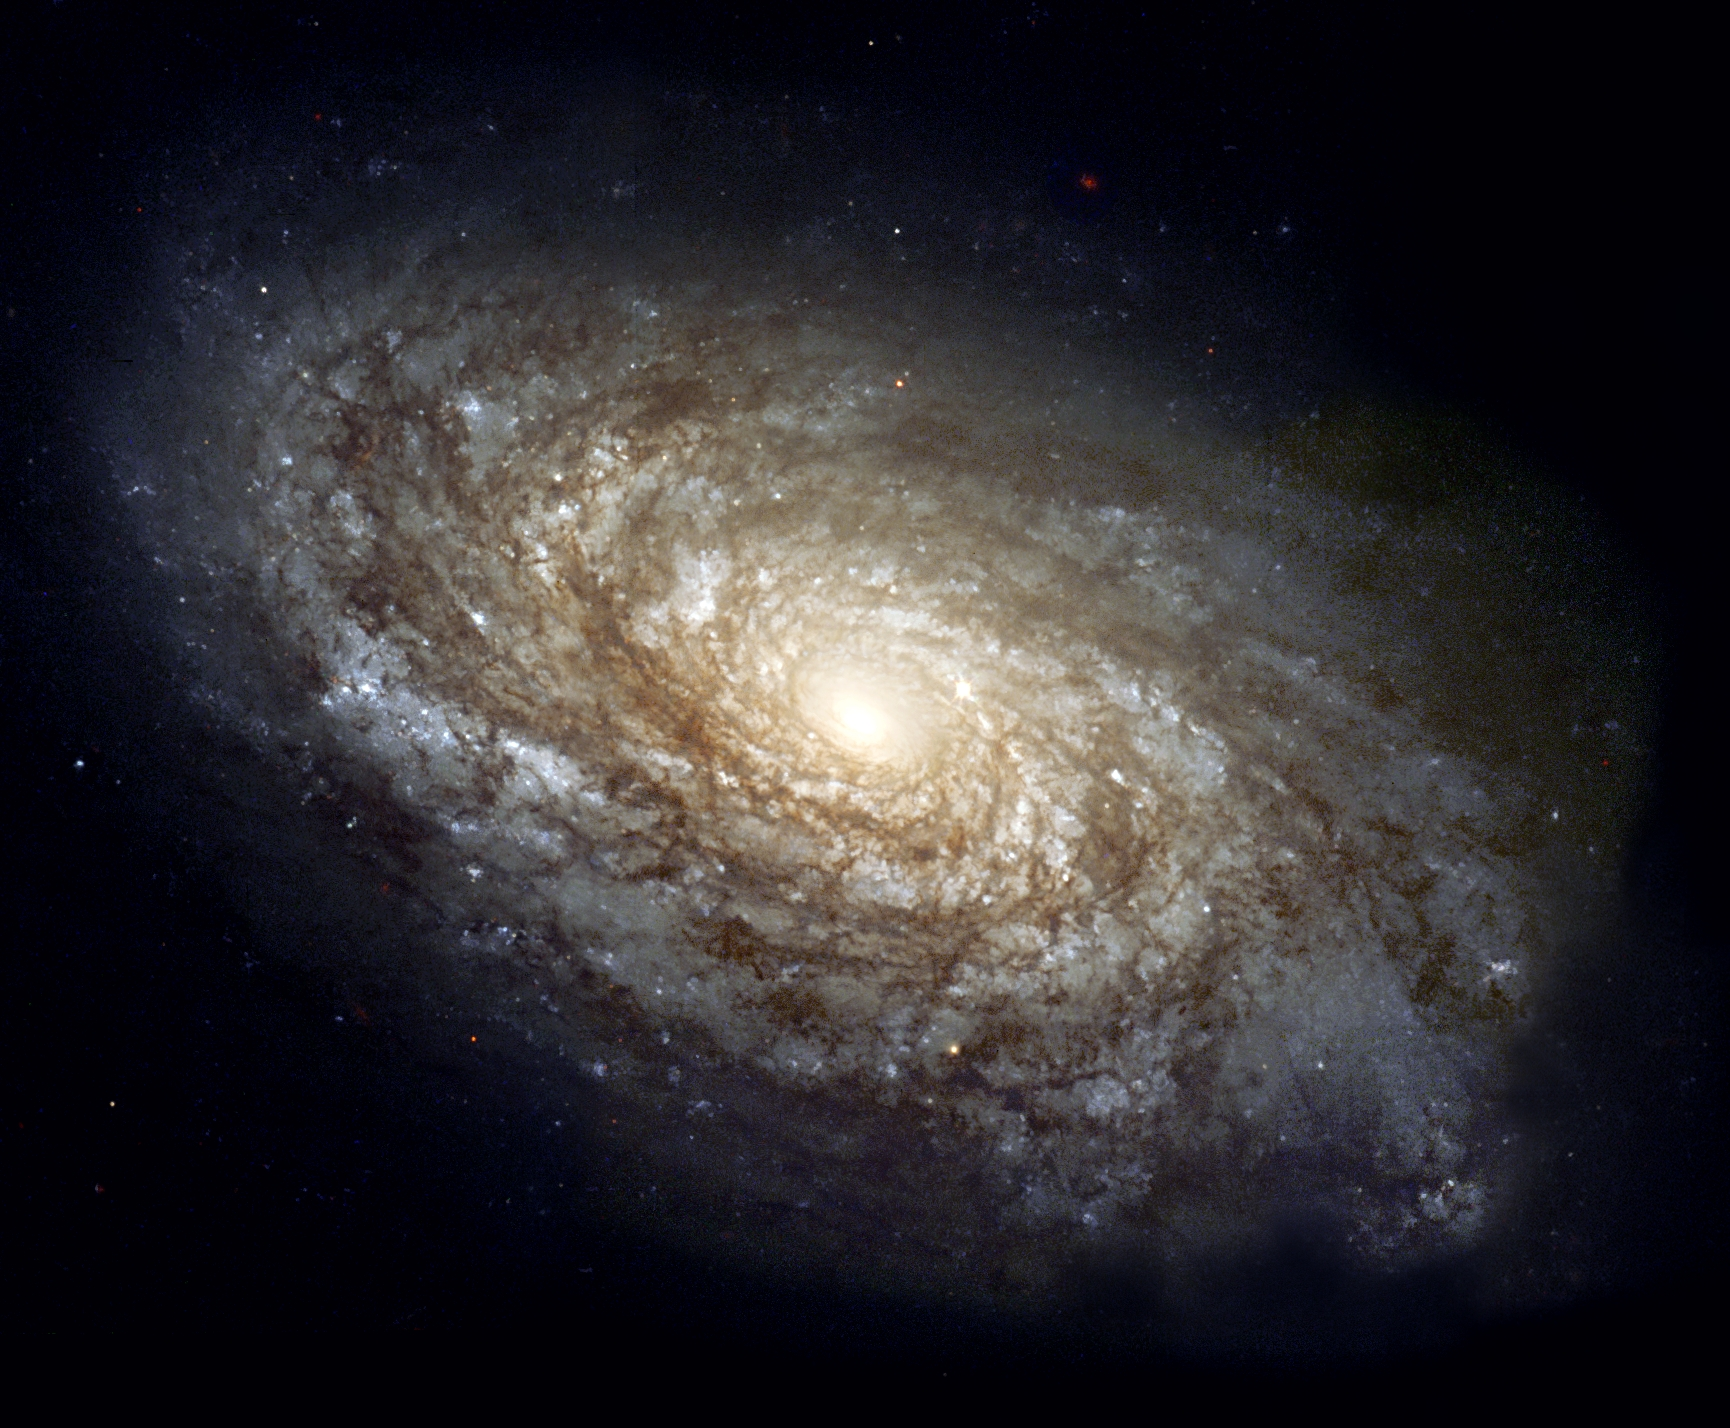
\includegraphics[width=\textwidth]{figure_1.jpg}
  %\caption{This is my caption.}
}

%%%%%%%%%%%%%%%%%%%%%%%%%%%%%%%%%%%%%%%%%%%%%%%%%%%%%%%%

\headerbox{What is our first model?}{name=model_1,column=0,below=box1%,above=bottom
}{Lorem ipsum dolor sit amet, consectetur adipiscing elit, sed do eiusmod tempor incididunt ut laboqu ~\cite{1}
\begin{equation}
    %\pdifff{x}{t} 
    \ddot{x}\; = - v_0 \pdiff{\xi}{x}(x,t/\tau).  \label{eq-newton}
\end{equation}
Lorem ipsum dolor sit amet, consectetur adipiscing elit, sed do eiusmod tempor incididunt ut laboqu ~\cite{2}
 $\langle e_k \rangle$ and mean square displacement $\sigma^2_x$
\begin{columns}
    \column{0.5\textwidth}
    \begin{equation}
    \langle e_k(t) \rangle  \propto v_0^2 \tau t,
    \end{equation}
    \column{0.5\textwidth}
    \begin{equation}
    \sigma_x^2(t) \propto v_0^2 \tau  t^3,
    \end{equation}
\end{columns}
Lorem ipsum dolor sit amet, consectetur adipiscing elit, sed do eiusmod tempor incididunt ut laboqu ~\cite{3} Lorem ipsum dolor sit amet, consectetur adipiscing elit, sed do eiusmod tempor incididunt ut laboqu ~\cite{3} Lorem ipsum dolor sit amet, consectetur adipiscing elit, sed do eiusmod tempor incididunt ut laboqu. Lorem ipsum dolor sit amet, consectetur adipiscing elit, sed do eiusmod tempor incididunt ut laboqu
}


%%% Box 2 %%%%%%%%%%%%%%%%%%%%%%%%%%%%%%%%%%%%%%%%%%%%%%%%%%%%%%%%%%%%%%%%%%%%%
\headerbox{What is our second model?}{name=model_2,column=1,below=abstract%,above=bottom
}{Lorem ipsum dolor sit amet, consectetur adipiscing elit, sed do eiusmod tempor incididunt ut labore et dolore magna aliqua. Ut enim ad minim veniam, quis nostrud exercitation ullamco laboris nisi ut aliquip 
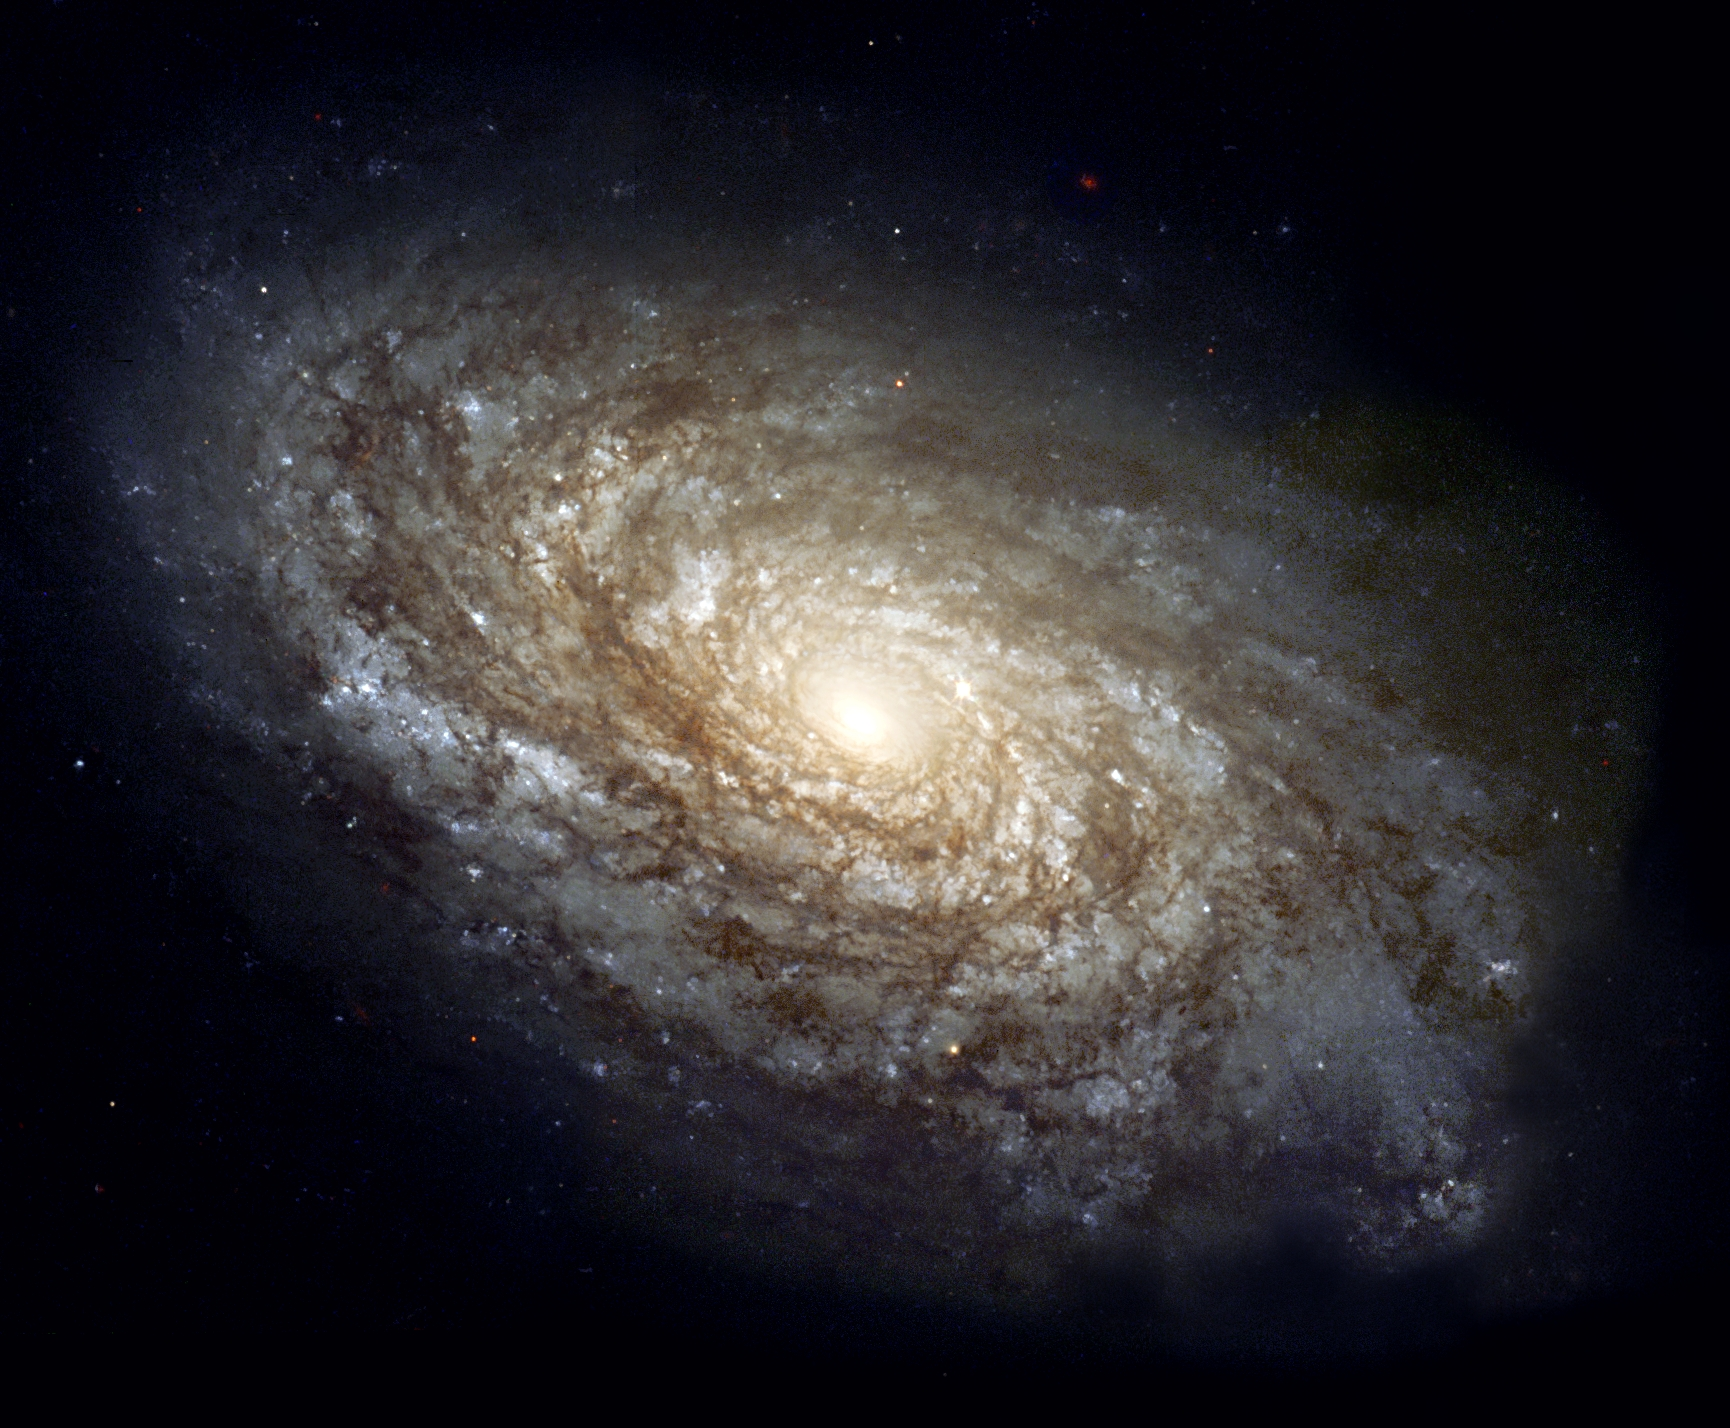
\includegraphics[width=\textwidth]{figure_1.jpg}
ex ea commodo consequat. Duis aute irure dolor in reprehenderit in voluptate velit esse cillum dolore eu fugiat nulla pariatur. Excepteur sint occaecat cupidatat non proident, sunt in culpa qui officia deserunt mollit anim id est laborum.
} 

\headerbox{Conclusions}{name=conclusions,column=1,below=model_2}{  ex ea commodo consequat. Duis aute irure dolor in reprehenderit in voluptate velit esse cillum dolore eu fugiat nulla pariatur. 
%\begin{figure}[t]
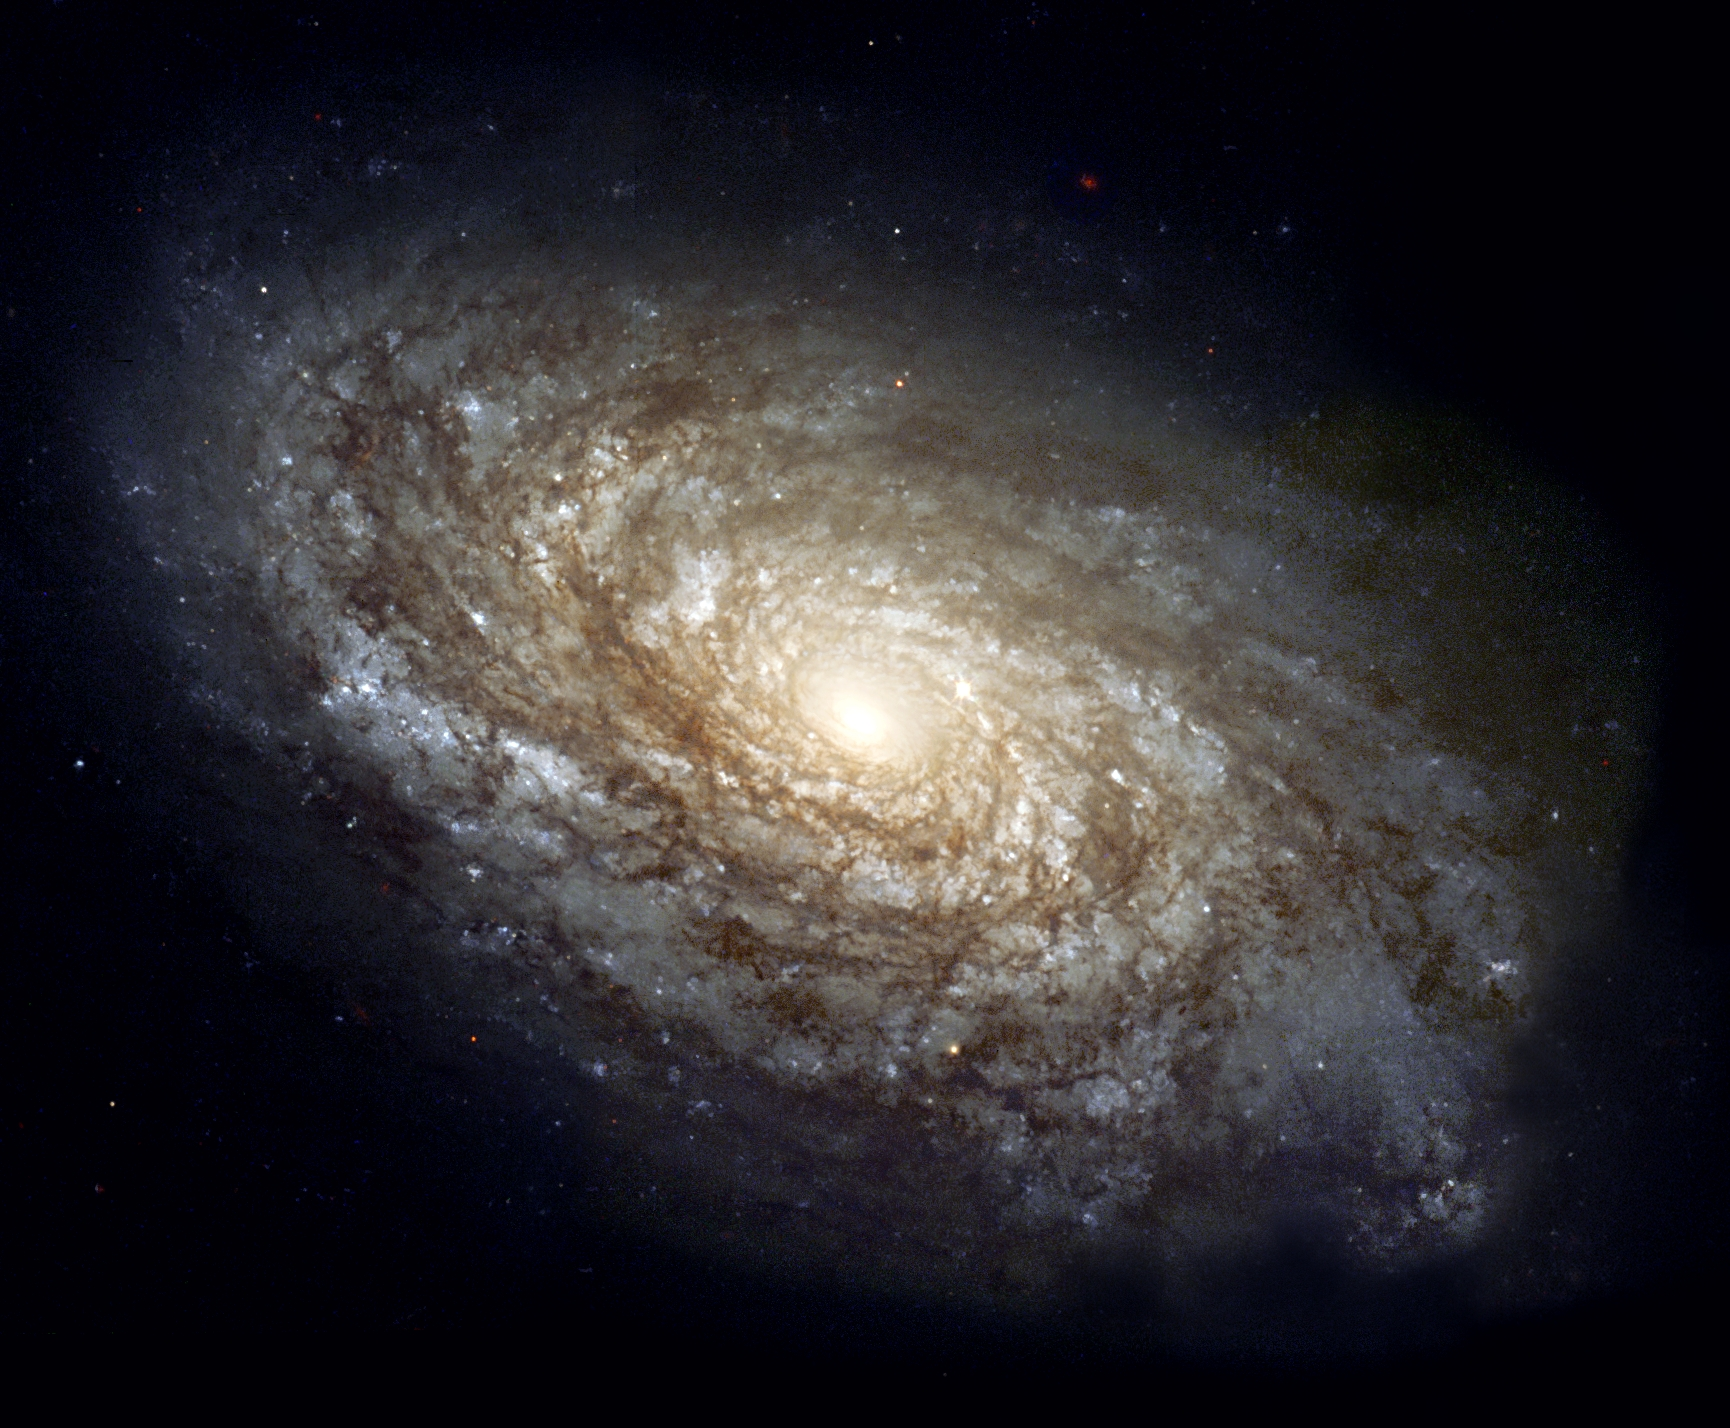
\includegraphics[width=0.5\textwidth]{figure_1.jpg}
%\caption{This is my caption.}
%\end{figure}

Excepteur sint occaecat cupidatat non proident, sunt in culpa qui officia deserunt mollit anim id est laborum.}

\headerbox{References}{name=references,column=0,below=conclusions, span=2}{

\renewcommand{\section}[2]{}
\begin{thebibliography}{9}
\bibitem{Topinka2001} M. A. Topinka, B. J. LeRoy, R. M. Westervelt, S. E. J. Shaw, R. Fleischmann, E. J. Heller, K. D. Maranowski, and A. C.
Gossard, Nature (London) {\bf 410}, 183 (2001).
\bibitem{Patsyk2020} A. Patsyk, U. Sivan, M. Segev, and M. A. Bandres, Nature
(London) {\bf 583}, 60 (2020).
\bibitem{Kaplan2002} L. Kaplan, Phys. Rev. Lett. {\bf 89}, 184103 (2002).
\end{thebibliography}

}

\end{poster}
\end{document}
